\documentclass[../main.tex]{subfiles}

\begin{document}

\section{DIS, nucleon structuur, PDF's}%
\label{sec:dis_nucleon_structuur_pdf_s}

\subsection{Diep inelastische verstrooiing}%
\label{sub:diep_inelastische_verstrooiing}

\begin{figure}[h]
    \centering
    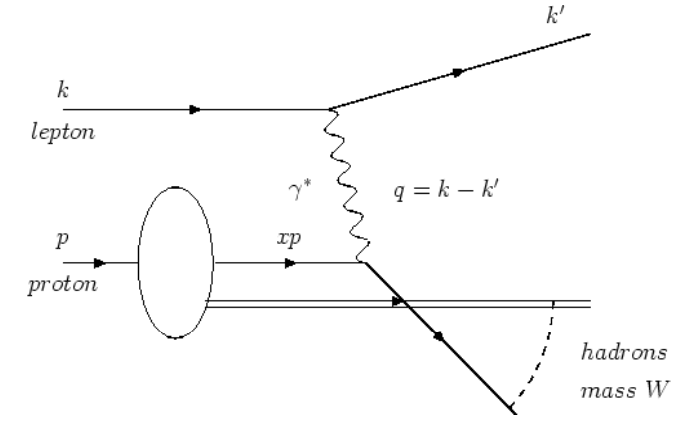
\includegraphics[width=0.8\linewidth]{DIS_nucleon_strutuur_pdf/diep_in_ver.png}
    \caption{Diep inelastische verstrooiing van een proton en een lepton}%
    \label{fig:diep_in_ver}
\end{figure}

Bij deze verstrooiing zal de kinetische energie van het lepton veel hoger zijn dan de massa van proton. Zo is het mogelijk om de inwendige structuur van het proton te gaan bekijken. De reden waarom we dit kunnen doen is omdat bij deze hoge energieën de golflengte van het foton veel kleiner zal zijn dan de grote van het proton. In dit geval werken we met een foton wat een groot voordeel is omdat we de vertices in dit diagram heel goed kunnen beschrijven en het lepton is een elementair deeltje. De enige onbekende in dit systeem is dus de inwendige structuur van het proton. De reden waarom het zo lang heeft geduurd voor we proton bundels zijn beginnen gebruiken is omdat niet alle massa in de valentie quarks van het proton zullen zitten wat het allemaal veel ingewikkelder maakt. Om met het LHC nauwkeurige metingen te kunnen uitvoeren moeten we veel meer statistiek (meer events) hebben.\\
De kinetiek van het proces schematisch weergegeven in figuur \ref{fig:diep_in_ver} kan makkelijk neergeschreven worden. Een parton (quark) van een proton met 4moment $xp$ zal een energie $q$ absorberen van het foton en een vrij deeltje worden.
\begin{equation}
    \begin{aligned}
        \label{eq:parton_foton_abs}
        \text{voor absorptie: }(xp+q)^2 &= m_{parton}^2 \approx 0\\
                                        &=x^2p^2+2xpq+q^2\\
                                        &=2xp+q^2\\
                          \Rightarrow x &=- \frac{-q^2}{2pq} = \frac{Q^2}{2pq} 
    \end{aligned}
\end{equation}
Het enige deeltje dat in staat zal zijn om een foton met energie $q$ te absorberen moet een impulsfractie $x$, zoals berekent in (\ref{eq:parton_foton_abs}), hebben van het proton. Met andere woorden hebben we een filter op welke partonen we willen waarnemen. Deze fractie is Lorentz invariant en dimensieloos. Een andere Lorentz invariante grootheid in dit proces is $y=\frac{q\cdot p}{k\cdot p}$. Deze geeft de fractie van het electron dat gedragen wordt door het foton.\\
Verder uitgewerkt op een vast target hebben we als 4 momenta:
\begin{equation}
    \begin{aligned}
        \label{eq:4_momenta_dis}
        k=
        \begin{pmatrix}
            E\\
            0\\
            0\\
            E
        \end{pmatrix},
        p=
        \begin{pmatrix}
            m_p\\
            0\\
            0\\
            0
        \end{pmatrix},
        k'=
        \begin{pmatrix}
            E'\\
            0\\
            E'\sin\theta\\
            E'\cos\theta
        \end{pmatrix},
        p_h=
        \begin{pmatrix}
            E_h\\
            p_{xh}\\
            p_{yh}\\
            p_{zh}\\
        \end{pmatrix}
    \end{aligned}
\end{equation}
De aannames dat we hier hebben gedaan zijn:
\begin{itemize}
    \item elektron beweegt langs de z-as
    \item door hoge energieën zien we het elektron als massaloos: $|E_e|=|p_{ze}|$
    \item het elektron verstrooit in het yz-vlak
    \item De hadronische finale toestand is de som van alle uitkomende deeltjes samen
\end{itemize}
De invariante massa van dit systeem is $W=\sqrt{E_H^2-\vec{p}^2_h}\geq m_p$. Het is mogelijk maar zeldzaam dat de geabsorbeerde energie kan verdeelt worden onder alle andere partons om zo een proton uit te komen. Dit is een elastische verstrooiing en $W=m_p$. In alle andere gevallen breekt het parton los van de rest en hebben we een inelastische verstrooiing met $W>m_p$.\\
Dit systeem heeft 8 vrijheidsgraden (voor zowel $k'$ als $p_h$ 1 voor de energie en 3 voor de hoeken). Eén van deze vrijheidsgraden valt weg vanwege de massa van het elektron dat verwaarloost wordt, nog 4 vallen weg door het behoud van energie en impuls en ten laatste valt er nog 1 weg door azimutale symmetrie. Zo houden we uiteindelijk nog 2 vrijheidsgraden over. De 2 makkelijkst te kiezen variabelen zijn $E'$ en $\theta$. Het probleem hierbij is dat deze niet Lorentz invariant zijn. Deze variabelen kunnen wel omgevormd worden naar $x$ en $y$ die dit wel zijn.
\begin{equation}
    \begin{aligned}
        \label{eq:etheta_naanr_xy}
        \begin{matrix}
            Q^2 & = & -(k-k')^2                 & \approx   & 2EE'(1-\cos\theta) \\
            x   & = & -\frac{q^2}{2p\cdot q}    & =         & \frac{EE'(1-\cos\theta)}{(E-E')m_p} \\
            y   & = & -\frac{q\cdot p}{k\cdot p}& =         & \frac{E-E'}{E} \\
        \end{matrix}
    \end{aligned}
\end{equation}

\subsection{Experimenten}%
\label{sub:experimenten}

\begin{figure}[h]
    \centering
    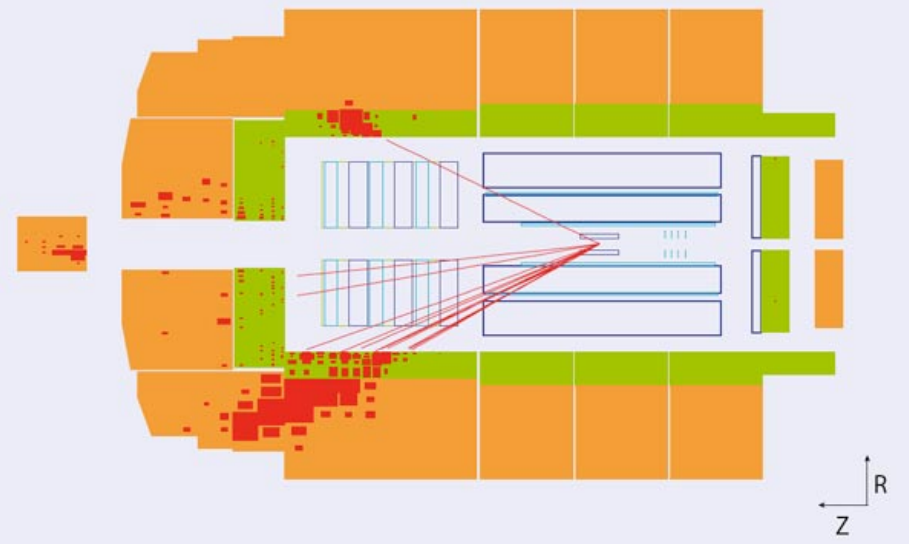
\includegraphics[width=0.6\linewidth]{DIS_nucleon_strutuur_pdf/hera.png}
    \caption{HERA experiment}%
    \label{fig:hera}
\end{figure}

De beste vaste target machines voor precisie zijn $e^+e^-$ colliders. Op deze machines zijn ook voor het eerst de quarks gezien. In het CERN hadden ze eerst een proton collider gemaakt en dachten dat ze de boot gemist hebben. Wat ze gedaan hebben is de protonen op een target insturen en daar komen massas pionen uit. Als je deze lang genoeg meeneemt gaan die vervallen naar muonen met een levensduur van de orde $10^{-8}$s en zo verkrijgen we een muon bundel. Omdat dit tertiaire deeltjes zijn gaat de densiteit van de deeltjes veel lager liggen en zullen een vrij breed energiespectrum hebben. Hetzelfde kan gedaan worden voor neutrino's.\\
Er zijn ook colliders waar 2 deeltjes bundels op elkaar worden afgestuurd. Een voorbeeld van de waargenomen deeltjes is in figuur \ref{fig:hera} gegeven van het HERA experiment. Hier is het duidelijk dat de elektronen van links zullen komen. Dit omdat de inkomende energie van het proton veel hoger is dan dat van het elektron en de uitgaande deeltjes van de collisie gaan wegens behoud van impuls via de linker kant de detector verlaten.\\
Als je zo een extravagant experiment zoals het LHC maakt is 1 van de eerste dingen die je doet het onderzoeken van het  kinematisch bereik van dat experiment. In figuur \ref{fig:kin_bereik} wordt $Q^2$ in functie van $x$ geplot van verschillend colliders.

\begin{figure}[h]
    \centering
    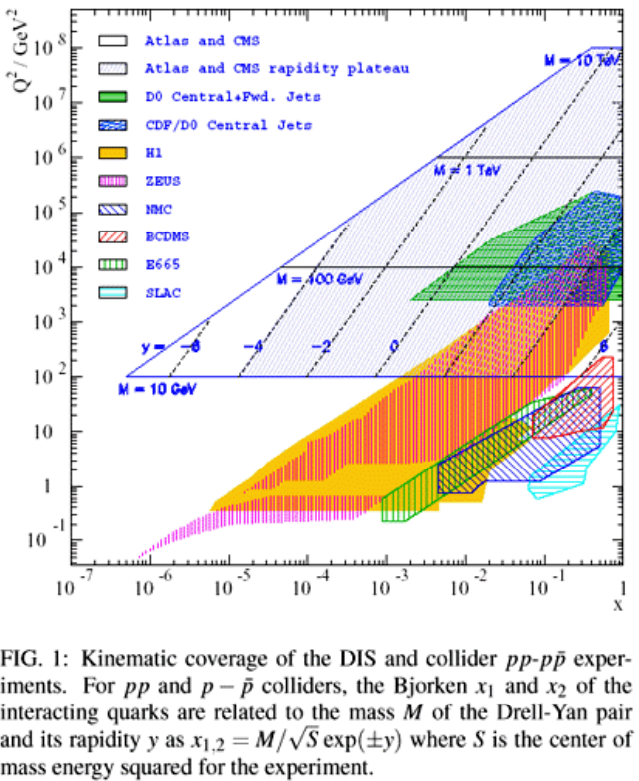
\includegraphics[width=0.8\linewidth]{DIS_nucleon_strutuur_pdf/kin_bereik.png}
    \caption{Kinematisch bereik}%
    \label{fig:kin_bereik}
\end{figure}

\subsection{Cross section}%
\label{sub:cross_section}

De werkzame doorsnede van deze DIS experimenten wordt gegeven door:
\begin{equation}
    \begin{aligned}
        \label{eq:dis_werkzame_doorsnede}
        \frac{d^2\sigma^{e,N}}{dxdy} = \frac{4\pi\alpha^2s}{Q^4} [xy^2F_1^{eN}+(1-y)F_2^{eN}]
    \end{aligned}
\end{equation}
met $F_1$ en $F_2$ de structuur functies. Het is logisch dat er in deze werkzame doorsnede een $\alpha^2$ afhankelijkheid verwerkt zit omdat deze interactie verloopt via de elektromagnetische interactie en dus 2 vertices heeft die elk een $\alpha$ toedragen. En de waarschijnlijkheid dat we de impulsfractie $x$ vinden van het parton wordt gegeven door die structuur functies $F_1$ en $F_2$. Het zijn deze dus die alle informatie bevatten. We zien dat de structuur functies afhangen van zowel $x$ als $Q^2$, $F_i(x, Q^2)$. Zo weten we direct dat dit geen puntdeeltjes kunnen zijn omdat we anders geen afhankelijkheid zouden hebben van $Q^2$.

\end{document}
